
\section{Bedienoberfläche}

Hier sind die Skizzen/Prototypen der Bedienoberflächen dargestellt. Außerdem sind auch die Zusammenhänge zwischen denen dargestellt.

\newcounter{gui}\setcounter{gui}{10}

\begin{description}[leftmargin=5em, style=sameline]	
	\begin{lhp}{gui}{GUI}{gui:graph}
		\item[Name:] Zusammenhänge
		\item[Beschreibung:] Zusammenhänge zwischen GUI-Ansichten.
		\item[Relevante Systemfunktionen:] Alle
		\item[Abbildungen:] \ref{gui:zusammenhang}
	\end{lhp}
\end{description}

\begin{description}[leftmargin=5em, style=sameline]	
	\begin{lhp}{gui}{GUI}{gui:launch}
		\item[Name:] Startbildschirm
		\item[Beschreibung:] Startbildschirm der erscheint, wenn man das Programm startet.
		\item[Relevante Systemfunktionen:] \ref{funk:zugriff}
		\item[Abbildungen:] \ref{gui:start}
	\end{lhp}
\end{description}

\begin{description}[leftmargin=5em, style=sameline]	
	\begin{lhp}{gui}{GUI}{gui:anmelden}
		\item[Name:] Vorraum-Interface
		\item[Beschreibung:] Interface für Anmeldung.
		\item[Relevante Systemfunktionen:] \ref{funk:zugriff}
		\item[Abbildungen:] \ref{gui:login}
	\end{lhp}
\end{description}

\begin{description}[leftmargin=5em, style=sameline]	
	\begin{lhp}{gui}{GUI}{gui:registrieren}
		\item[Name:] Registrierungs-Interface
		\item[Beschreibung:] Interface das erscheint, wenn man einen neuen Benutzer registrieren will.
		\item[Relevante Systemfunktionen:] \ref{funk:accountverw}
		\item[Abbildungen:] \ref{gui:register}
	\end{lhp}
\end{description}

\begin{description}[leftmargin=5em, style=sameline]	
	\begin{lhp}{gui}{GUI}{gui:launch}
		\item[Name:] Auswahlbildschirm
		\item[Beschreibung:] Entscheidungsbildschirm, mit Optionen zum Spielstart, Daten ändern und Bestenliste ansehen
		\item[Relevante Systemfunktionen:] \ref{funk:zugriff}
		\item[Abbildungen:] \ref{gui:menü}
	\end{lhp}
\end{description}

\begin{description}[leftmargin=5em, style=sameline]	
	\begin{lhp}{gui}{GUI}{gui:change}
		\item[Name:] Accountoptionen
		\item[Beschreibung:] Interface zum ändern der Benutzerdaten.
		\item[Relevante Systemfunktionen:] \ref{funk:accountverw}
		\item[Abbildungen:] \ref{gui:daten}
	\end{lhp}
\end{description}

\begin{description}[leftmargin=5em, style=sameline]	
	\begin{lhp}{gui}{GUI}{gui:liste}
		\item[Name:] Bestenliste
		\item[Beschreibung:] Anzeige der Bestenliste.
		\item[Relevante Systemfunktionen:] \ref{funk:bestenliste}
		\item[Abbildungen:] \ref{gui:bestenliste}
	\end{lhp}
\end{description}

\begin{description}[leftmargin=5em, style=sameline]	
	\begin{lhp}{gui}{GUI}{gui:opt}
		\item[Name:] Spieloptionen
		\item[Beschreibung:] Entscheidungsbildschirm ob mit Bots oder ohne gespielt wird.
		\item[Relevante Systemfunktionen:] \ref{funk:bots}
		\item[Abbildungen:] \ref{gui:option}
	\end{lhp}
\end{description}

\begin{description}[leftmargin=5em, style=sameline]	
	\begin{lhp}{gui}{GUI}{gui:niv}
		\item[Name:] Niveau-Auswahl
		\item[Beschreibung:] Entscheidungsbildschirm ob mit schweren oder einfachen Bots gespielt wird.
		\item[Relevante Systemfunktionen:] \ref{funk:bots}
		\item[Abbildungen:] \ref{gui:niveau}
	\end{lhp}
\end{description}

\begin{description}[leftmargin=5em, style=sameline]	
	\begin{lhp}{gui}{GUI}{gui:lob}
		\item[Name:] Lobby
		\item[Beschreibung:] Lobby in der man anderen Spielen beitreten kann oder selbst erstellen kann.
		\item[Relevante Systemfunktionen:] \ref{funk:spielraum} \ref{funk:chat}
		\item[Abbildungen:] \ref{gui:lobby}
	\end{lhp}
\end{description}

\begin{description}[leftmargin=5em, style=sameline]	
	\begin{lhp}{gui}{GUI}{gui:room}
		\item[Name:] Spielraum
		\item[Beschreibung:] Spielraum in dem das Spiel stattfindet.
		\item[Relevante Systemfunktionen:] \ref{funk:spielverw} \ref{funk:chat}
		\item[Abbildungen:] \ref{gui:raum}
	\end{lhp}
\end{description}


\begin{figure}
	\centering
	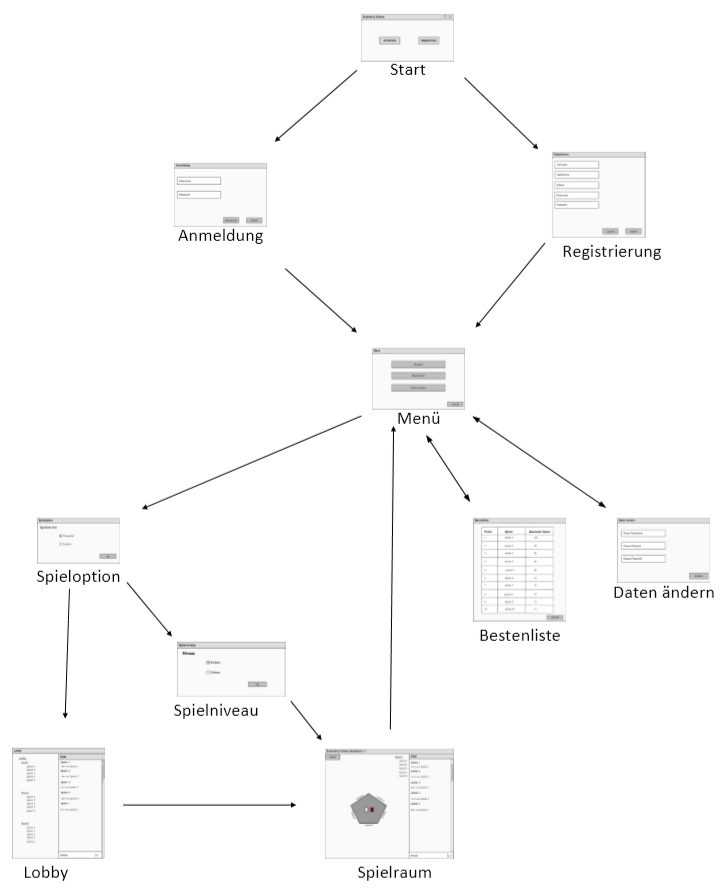
\includegraphics[width=0.9\textwidth]{img/Graph}
	\caption{Darstellung der Zusammenhänge zwischen GUI-Ansichten.}
	\label{gui:zusammenhang}
\end{figure}

\begin{figure}
	\centering
	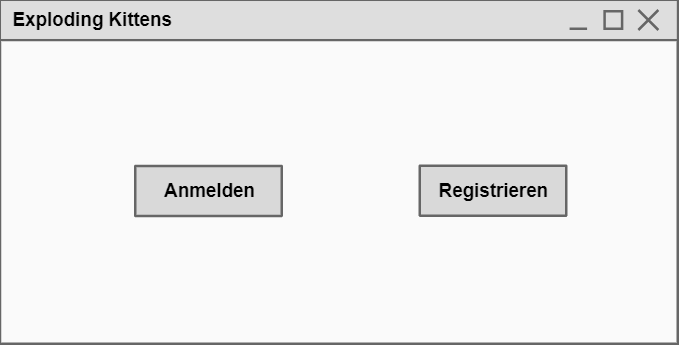
\includegraphics[width=0.5\textwidth]{img/Launch}
	\caption{Skizze für das Startfenster des Programms.}
	\label{gui:start}
\end{figure}

\begin{figure}
	\centering
	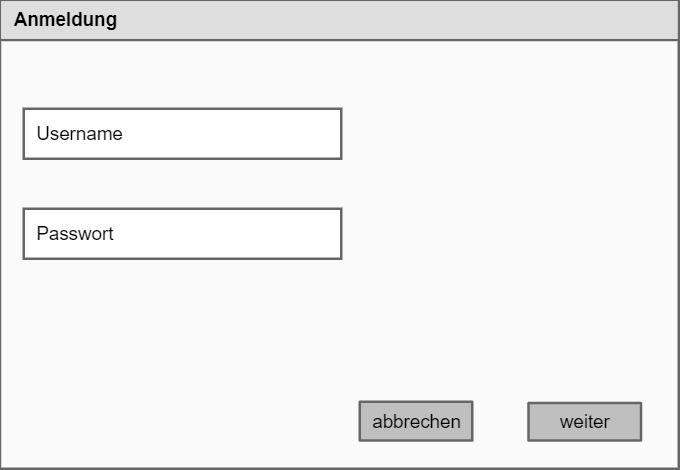
\includegraphics[width=0.5\textwidth]{img/Anmelden}
	\caption{Skizze für das Anmeldefenster.}
	\label{gui:login}
\end{figure}

\begin{figure}
	\centering
	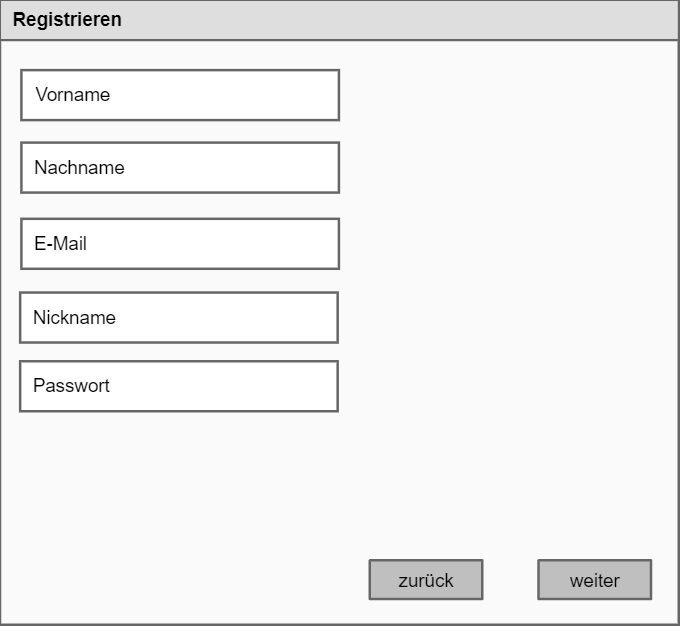
\includegraphics[width=0.5\textwidth]{img/Registrieren}
	\caption{Skizze für das Registrierungsfenster.}
	\label{gui:register}
\end{figure}

\begin{figure}
	\centering
	\includegraphics[width=0.5\textwidth]{img/Menü}
	\caption{Skizze für das Auswahlmenü.}
	\label{gui:menü}
\end{figure}

\begin{figure}
	\centering
	\includegraphics[width=0.5\textwidth]{img/Daten ändern}
	\caption{Skizze für das Fenster zum ändern der Benutzerdaten.}
	\label{gui:daten}
\end{figure}

\begin{figure}
	\centering
	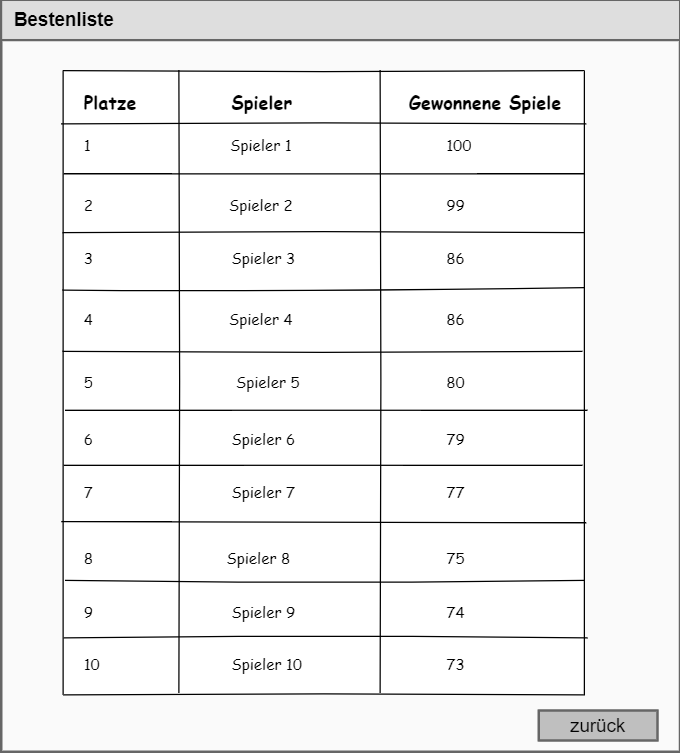
\includegraphics[width=0.5\textwidth]{img/Bestenliste}
	\caption{Skizze für die Bestenliste.}
	\label{gui:bestenliste}
\end{figure}

\begin{figure}
	\centering
	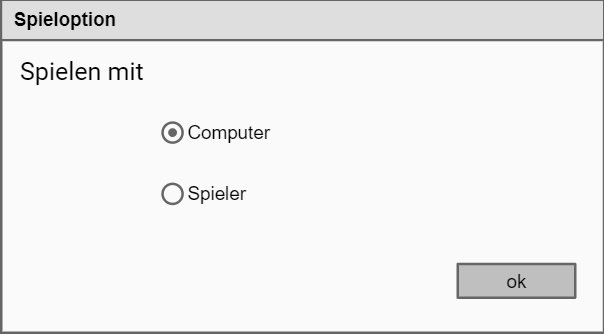
\includegraphics[width=0.5\textwidth]{img/Spieloption}
	\caption{Skizze für das Auswahlfenster zwischen Bots und echten Spielern.}
	\label{gui:option}
\end{figure}

\begin{figure}
	\centering
	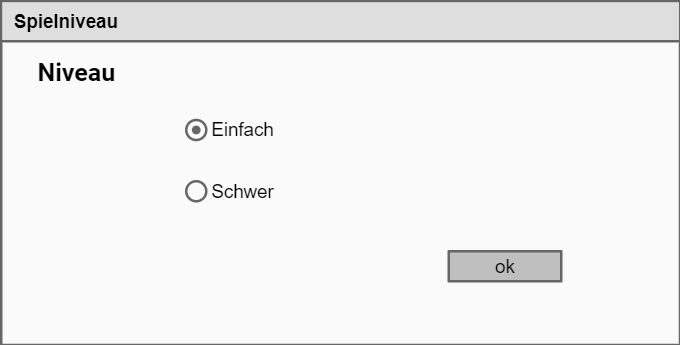
\includegraphics[width=0.5\textwidth]{img/Niveau}
	\caption{Skizze für den Auswahlbildschirm der Bot Schwierigkeit.}
	\label{gui:niveau}
\end{figure}

\begin{figure}
	\centering
	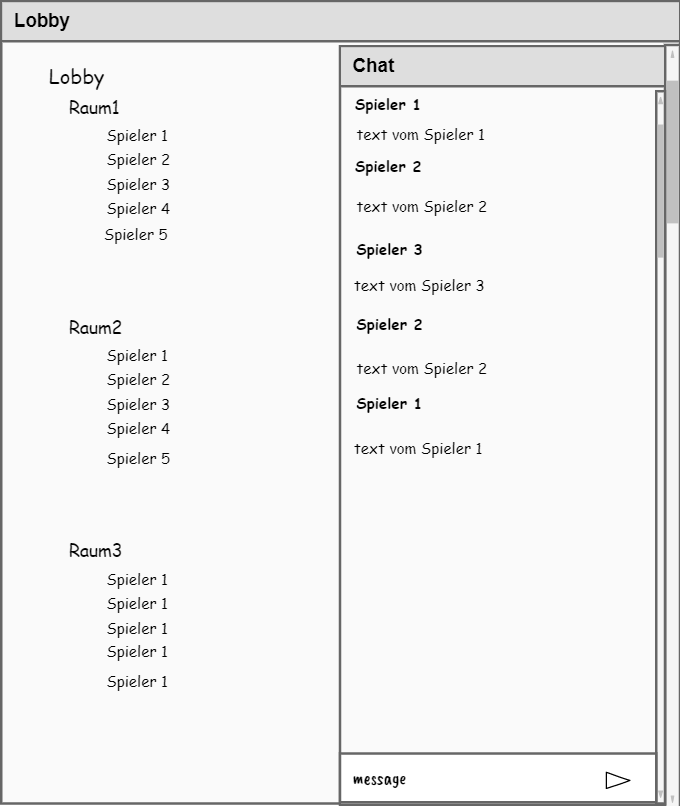
\includegraphics[width=0.5\textwidth]{img/Lobby}
	\caption{Skizze für die Lobby.}
	\label{gui:lobby}
\end{figure}

\begin{figure}
	\centering
	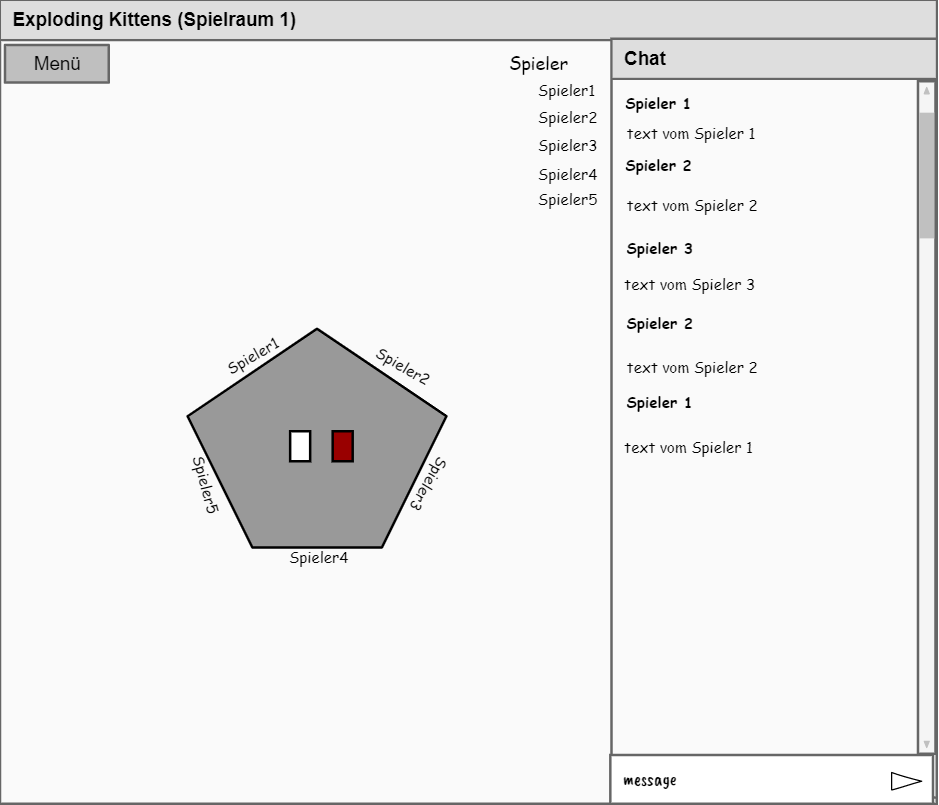
\includegraphics[width=0.5\textwidth]{img/Spielraum}
	\caption{Skizze für den Spielraum.}
	\label{gui:raum}
\end{figure}
